
%we use article class because we want to fully customize the page and dont use a cv template
\documentclass[10pt,A4]{article}


%----------------------------------------------------------------------------------------
%	ENCODING
%----------------------------------------------------------------------------------------

%we use utf8 since we want to build from any machine
\usepackage[utf8]{inputenc}

%----------------------------------------------------------------------------------------
%	LOGIC
%----------------------------------------------------------------------------------------

% provides \isempty test
\usepackage{xifthen}

%----------------------------------------------------------------------------------------
%	FONT
%----------------------------------------------------------------------------------------

\usepackage{hyperref}
\usepackage{xstring}

\hypersetup{
    colorlinks=false
}
% some tex-live fonts - choose your own

%\usepackage[defaultsans]{droidsans}
%\usepackage[default]{comfortaa}
%\usepackage{cmbright}
\usepackage[default]{raleway}
%\usepackage{fetamont}
%\usepackage[default]{gillius}
%\usepackage[light,math]{iwona}
%\usepackage[thin]{roboto}

% set font default
\renewcommand*\familydefault{\sfdefault}
\usepackage[T1]{fontenc}

% more font size definitions
\usepackage{moresize}


%----------------------------------------------------------------------------------------
%	PAGE LAYOUT  DEFINITIONS
%----------------------------------------------------------------------------------------

%debug page outer frames
%\usepackage{showframe}


%define page styles using geometry
\usepackage[a4paper]{geometry}

% for example, change the margins to 2 inches all round
\geometry{top=1.75cm, bottom=-.6cm, left=1.5cm, right=1.5cm}

%use customized header
\usepackage{fancyhdr}
\pagestyle{fancy}

%less space between header and content
\setlength{\headheight}{-5pt}


%customize entries left, center and right
\lhead{}
\chead{\small{Alex Ghiurau $\cdot$ Software Engineer $\cdot$ Oradea, Romania $\cdot$ \textcolor{sectcol}{\textbf{alex.ghiurau@gmail.com}} $\cdot$ +40 748 575 571}}
\rhead{}


%indentation is zero
\setlength{\parindent}{0mm}

%----------------------------------------------------------------------------------------
%	TABLE /ARRAY DEFINITIONS
%----------------------------------------------------------------------------------------

%for layouting tables
\usepackage{multicol}
\usepackage{multirow}

%extended aligning of tabular cells
\usepackage{array}

\newcolumntype{x}[1]{%
>{\raggedleft\hspace{0pt}}p{#1}}%


%----------------------------------------------------------------------------------------
%	GRAPHICS DEFINITIONS
%----------------------------------------------------------------------------------------

%for header image
\usepackage{graphicx}

%for floating figures
\usepackage{wrapfig}
\usepackage{float}
%\floatstyle{boxed}
%\restylefloat{figure}

%for drawing graphics
\usepackage{tikz}
\usetikzlibrary{shapes, backgrounds,mindmap, trees}


%----------------------------------------------------------------------------------------
%	Color DEFINITIONS
%----------------------------------------------------------------------------------------

\usepackage{color}

%accent color
\definecolor{sectcol}{RGB}{255,150,0}

%dark background color
\definecolor{bgcol}{RGB}{110,110,110}

%light background / accent color
\definecolor{softcol}{RGB}{225,225,225}


%============================================================================%
%
%
%	DEFINITIONS
%
%
%============================================================================%

\newcommand\AddAdditional[1]{%
  \StrLen{#1}[\MyStrLen]% we find the length of the string and store it in \MyStrLen
  \ifthenelse{\equal{\MyStrLen}{1}}% we compare the length of the string with 1
        {}{\larrow{bgcol} #1}}

%----------------------------------------------------------------------------------------
% 	HEADER
%----------------------------------------------------------------------------------------

% remove top header line
\renewcommand{\headrulewidth}{0pt}

%remove botttom header line
\renewcommand{\footrulewidth}{0pt}

%remove pagenum
\renewcommand{\thepage}{}

%remove section num
\renewcommand{\thesection}{}

%----------------------------------------------------------------------------------------
% 	ARROW GRAPHICS in Tikz
%----------------------------------------------------------------------------------------

% a six pointed arrow poiting to the left
\newcommand{\tzlarrow}{(0,0) -- (0.2,0) -- (0.3,0.2) -- (0.2,0.4) -- (0,0.4) -- (0.1,0.2) -- cycle;}

% include the left arrow into a tikz picture
% param1: fill color
%
\newcommand{\larrow}[1]
{\begin{tikzpicture}[scale=0.58]
	 \filldraw[fill=#1!100,draw=#1!100!black]  \tzlarrow
 \end{tikzpicture}
}

% a six pointed arrow poiting to the right
\newcommand{\tzrarrow}{ (0,0.2) -- (0.1,0) -- (0.3,0) -- (0.2,0.2) -- (0.3,0.4) -- (0.1,0.4) -- cycle;}

% include the right arrow into a tikz picture
% param1: fill color
%
\newcommand{\rarrow}
{
\begin{tikzpicture}[scale=0.7]
	\filldraw[fill=sectcol!100,draw=sectcol!100!black] \tzrarrow
 \end{tikzpicture}
}



%----------------------------------------------------------------------------------------
%	custom sections
%----------------------------------------------------------------------------------------

% create a coloured box with arrow and title as cv section headline
% param 1: section title
%
\newcommand{\cvsection}[1]
{
\colorbox{sectcol}{\mystrut \makebox[1\linewidth][l]{
\larrow{bgcol} \hspace{-8pt} \larrow{bgcol} \hspace{-8pt} \larrow{bgcol} \textcolor{white}{\textbf{#1}}\hspace{4pt}
}}\\
}

%create a coloured arrow with title as cv meta section section
% param 1: meta section title
%
\newcommand{\metasection}[2]
{
\begin{tabular*}{1\textwidth}{p{2.4cm} p{11cm}}
\larrow{bgcol}	\normalsize{\textcolor{sectcol}{#1}}&#2\\[12pt]
\end{tabular*}
}

%----------------------------------------------------------------------------------------
%	 CV EVENT
%----------------------------------------------------------------------------------------

% creates a stretched box as cv entry headline followed by two paragraphs about
% the work you did
% param 1:	event time i.e. 2014 or 2011-2014 etc.
% param 2:	event name (what did you do?)
% param 3:	institution (where did you work / study)
% param 4:	what was your position
% param 5:	some words about your contributions
% param 6:	some link
%
\newcommand{\cvevent}[7]
{
\vspace{14pt}
	\begin{tabular*}{1\textwidth}{p{2.3cm}  p{10.8cm} x{3.9cm}}
 \textcolor{bgcol}{#1}& \textbf{#2} & \vspace{2.5pt}\textcolor{sectcol} {#3}

	\end{tabular*}
\vspace{6pt}
	\begin{tabular*}{1\textwidth}{p{2.3cm} p{10.8cm} p{3.9cm}}
&		 \larrow{bgcol}  #4 & \\[3pt]
&		 \larrow{bgcol}  #5 & \\[6pt]
&		 \AddAdditional{#6} & \\[4pt]
& 		\AddAdditional{#7} &
	\end{tabular*}

}

% creates a stretched box as
\newcommand{\cveventmeta}[2]
{
	\mbox{\mystrut \hspace{87pt}\textit{#1}}\\
	#2
}

%----------------------------------------------------------------------------------------
% CUSTOM STRUT FOR EMPTY BOXES
%----------------------------------------- -----------------------------------------------
\newcommand{\mystrut}{\rule[-.3\baselineskip]{0pt}{\baselineskip}}

%----------------------------------------------------------------------------------------
% CUSTOM LOREM IPSUM
%----------------------------------------------------------------------------------------
\newcommand{\lorem}
{Lorem ipsum dolor sit amet, consectetur adipiscing elit. Donec a diam lectus.}



%============================================================================%
%
%
%
%	DOCUMENT CONTENT
%
%
%
%============================================================================%
\begin{document}


%use our custom fancy header definitions
\pagestyle{fancy}


%---------------------------------------------------------------------------------------
%	TITLE HEADLINE
%----------------------------------------------------------------------------------------
\vspace{-20.55pt}

% use this for multiple words like working titles etc.
%\hspace{-0.25\linewidth}\colorbox{bgcol}{\makebox[1.5\linewidth][c]{\hspace{46pt}\HUGE{\textcolor{white}{\textsc{Alex Ghiurău}} } \textcolor{sectcol}{\rule[-1mm]{1mm}{0.9cm}} \parbox[b]{5cm}{   \large{ \textcolor{white}{{IT Consultant}}}\\
% \large{ \textcolor{white}{{Resume}}}}
%}}

% use this for single words, e.g. CV or RESUME etc.
\hspace{-0.25\linewidth}\colorbox{bgcol}{\makebox[1.5\linewidth][c]{\HUGE{\textcolor{white}{\textsc{Alex Ghiurau}} } \textcolor{sectcol}{\rule[-1mm]{1mm}{0.9cm}} \HUGE{\textcolor{white}{\textsc{Resume}} } }}


%----------------------------------------------------------------------------------------
%	HEADER IMAGE
%----------------------------------------------------------------------------------------

\begin{figure}[H]
\begin{flushright}
	
\includegraphics[width=103pt]{qrcode}
	% 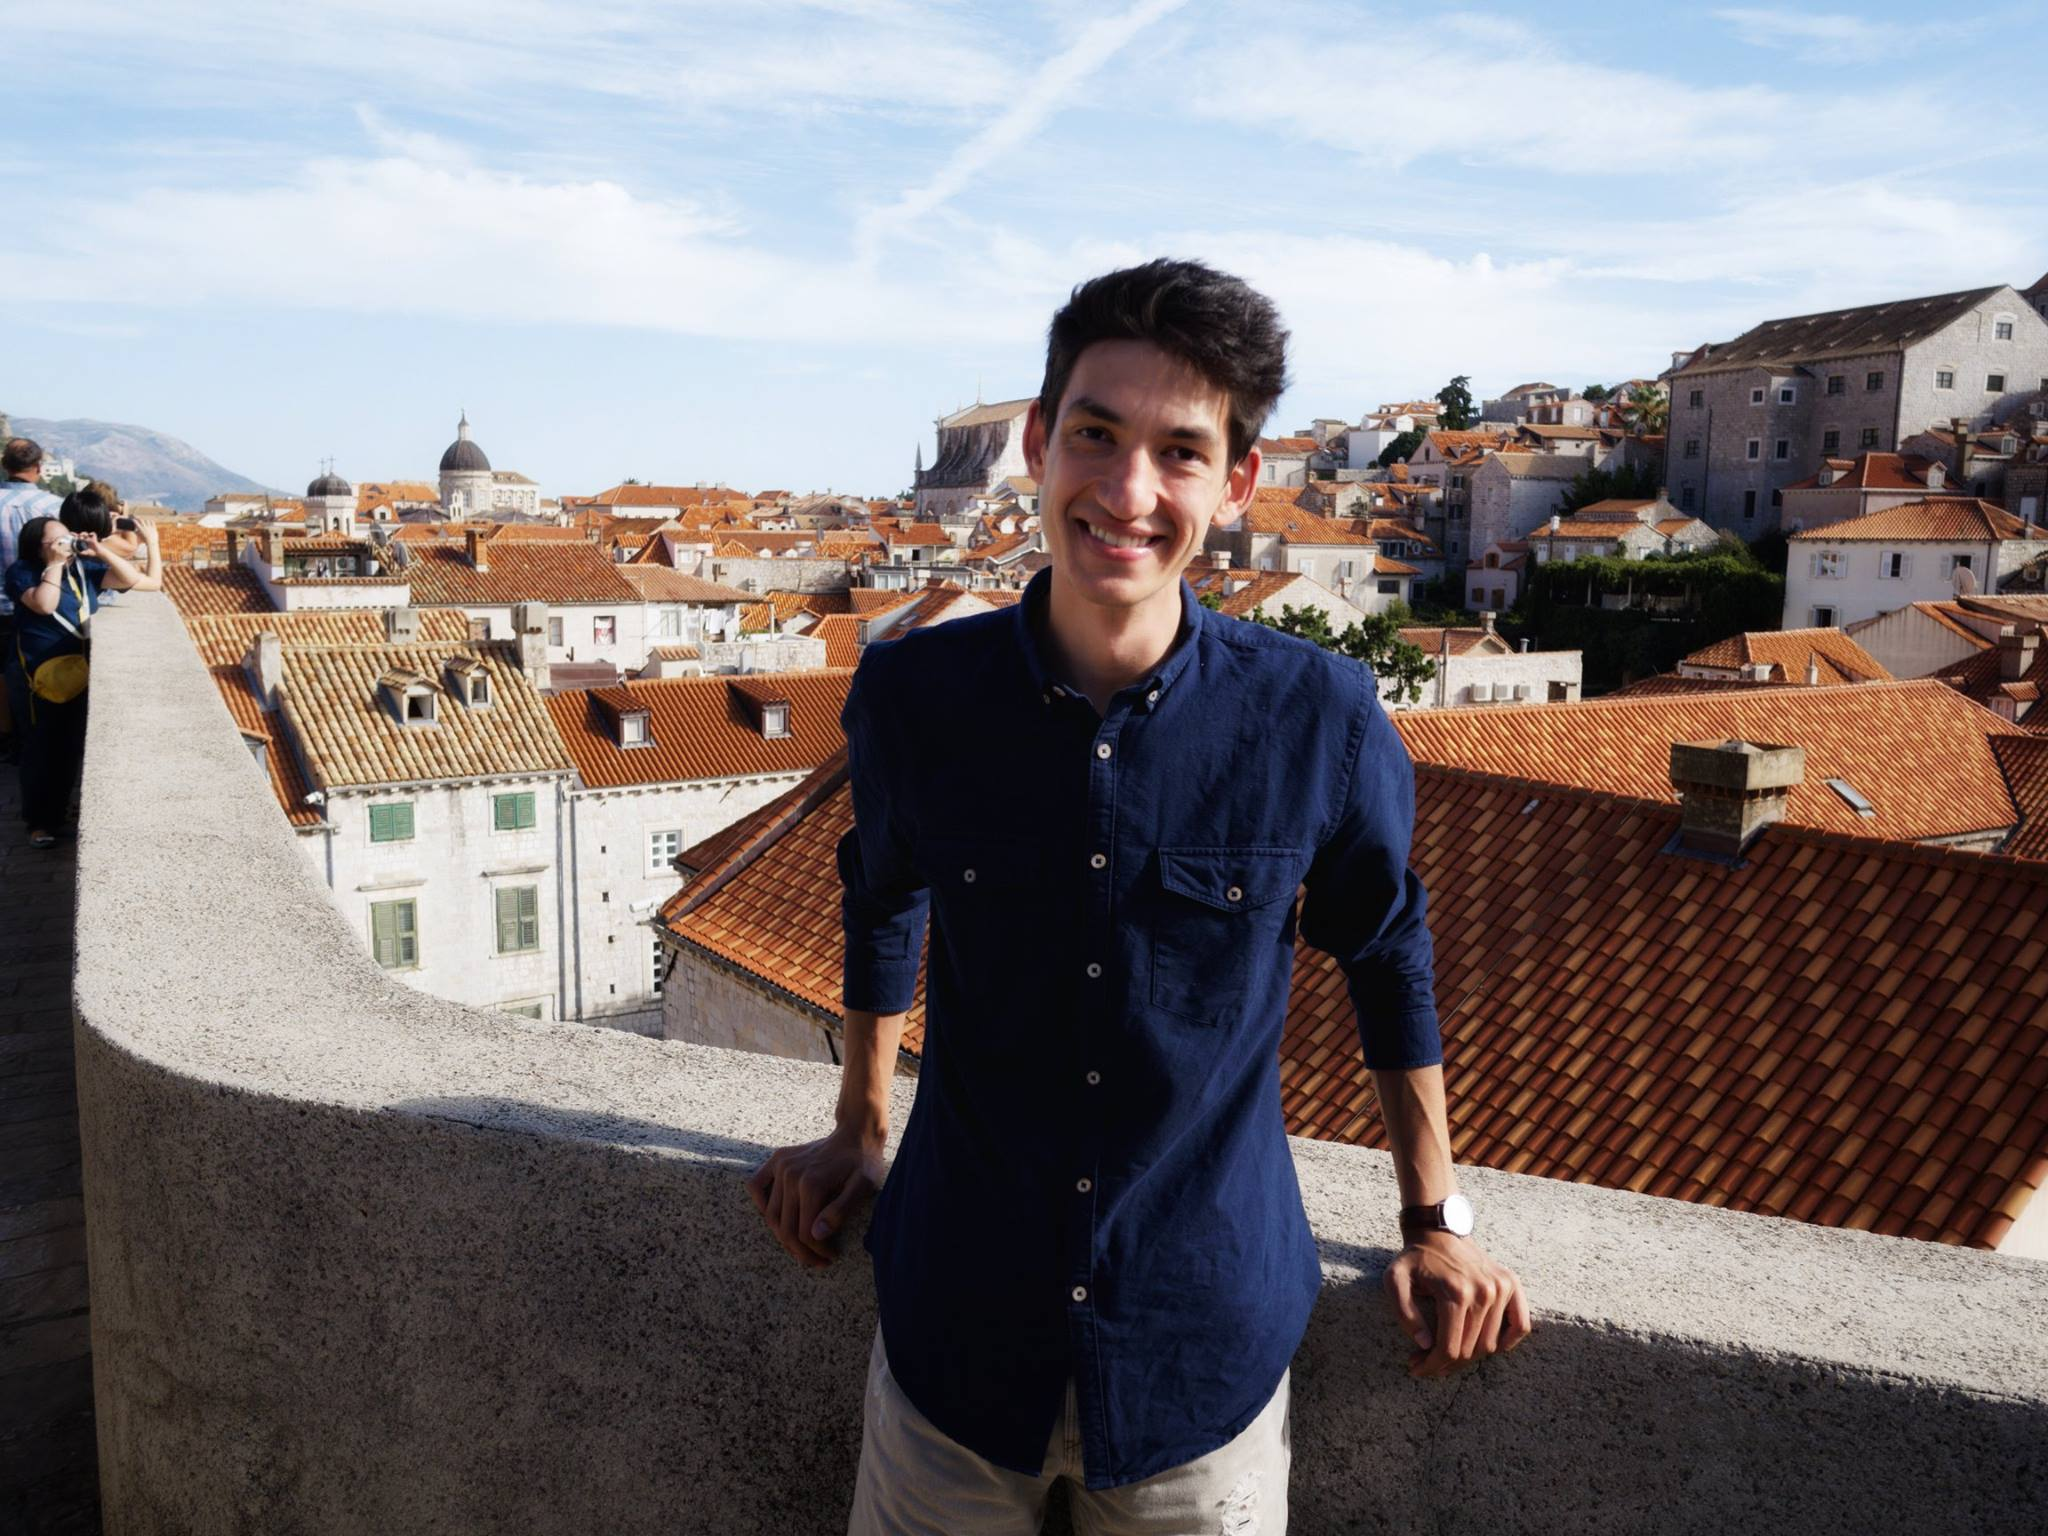
\includegraphics[trim= 320 130 460 210,clip,width=0.2\linewidth]{myfoto.jpg}	%trimming relative to image size!
\end{flushright}
\end{figure}

%---------------------------------------------------------------------------------------
%	QR CODE (optional)
%----------------------------------------------------------------------------------------
%\vspace{-136pt}
%\hspace{0.75\linewidth}
%
\includegraphics[width=103pt]{qrcode}
%\normalsize
%\vspace{88pt}

%---------------------------------------------------------------------------------------
%	META SECTION
%----------------------------------------------------------------------------------------

\vspace{-114pt}

\metasection{Status:}{Fullstack JS Engineer, B.Sc.Eng - Networking \& Telecommunications}
\metasection{Fields:}{Software Development, Teaching, Project Management, UX}
\metasection{Tech:}{Javascript - (React, NodeJS, Extjs), ReactNative, Electron, GraphQL, MySQL, PHP, Git, PhpStorm, Sourcetree, AWS - (S3, CloudWatch)}
\metasection{Loves:}{Music, Photography, Mountains, Books \& Tea}

\vspace{6pt}

%---------------------------------------------------------------------------------------
%	SUMMARAY (optional)
%----------------------------------------------------------------------------------------

%\cvsection{Summary}\\
% I am a networking \& telecommunications graduate (B.S.E) with project experience in the private sector. I worked at Digi Communications, also known as RCS \& RDS (romania communication systems - romania data systems), as a Tech Support for clients.

% Currently I develop a mobile application that replicates the main functionalities of the main webapp called Paymo (a Project Management SaaS app) with React Native so that we can target both main mobile platforms. I also love hiking into the mountains, taking photos of spectacular sceneries \& reading books.\\[-2pt]

%============================================================================%
%
%	CV SECTIONS AND EVENTS (MAIN CONTENT)
%
%============================================================================%

%---------------------------------------------------------------------------------------
%	EXPERIENCE
%----------------------------------------------------------------------------------------
\cvsection{Summary}
\\I hold a Bachelor of Science in Engineering with a specialization in Networking and Telecommunications. My professional background includes valuable project experience within the private sector.\\
\\During my tenure at Paymo, I dealt with lots of things, but the most recent one was build a mobile application. This project involved the utilization of technologies such as React Native, GraphQL, and various other tools.\\
\\After this, Paymo got aquired by Profitsolv and I cotinued working on various projects such as iOrion and built their mobile application using the technologies mentioned before, and then for other projects using React.\\
\\As a personal endeavor, I created a mobile radio application, Radio Aripi Spre Cer using React Native and NodeJS \\ - https://apple.co/430v2Nq. \\
\\Furthermore, I embraced the role of an educator. I led a class at the University Emanuel of Oradea, specializing in Advanced Concepts in Web Programming. This teaching experience has been especially rewarding and closely aligns with my professional interests.\\[-2pt]
\\In my leisure time, I find solace in reading books on weekends or whenever the opportunity arises. I am passionate about hiking and capturing photographs of breathtaking sceneries.\\[-2pt]

\textcolor{softcol}{\hrule}

\cvsection{Experience}

%
\cvevent{2022 - present}{Fullstack Javascript Engineer}{Profitsolv}
{Developed the mobile app iOrion (iOrion6) in ReactNative, an app for lawyers to manage their cases, clients, and appointments}
{Accelerated the development process in another project from the portfolio}
{Led a team and made architectural changes to a very old project, which resulted in a stability increase of the app, customer satisfaction, reduced costs, and increased revenue}

%
\cvevent{2017 - 2022}{Fullstack Javascript Engineer}{Paymo}
{Developed the mobile app (Paymo) that has the same functionality as the main web app using React Native, GraphQL \& other libraries}
{Created an onboarding progress tutorial for newly subscribed users using React}
{Developed a timer widget using Electron so that users can easily track time and add time entries from their desktop platforms}
{Implemented a Notifications Systems - a queued system that sends email notifications, in-app notifications, and mobile notifications (using Firebase) to concerned users using PHP Resque \& Redis}

%
\cvevent{2022 - 2024}{Teacher}{University Emanuel of Oradea}
{Designed a curriculum that covers fundamental and advanced concepts of React. This involves selecting appropriate textbooks, creating lecture materials, and designing hands-on projects that allow students to apply React concepts.}
{Conducted lectures, demonstrations, and coding sessions to teach students how to use React effectively.}
{Designed practical projects that enable students to apply React concepts in real-world scenarios.}

%
\cvevent{2022 - 2023}{Founder}{HyggeToday}
{Started a 'startup', wore many hats doing lots of things, conceptualized and refined the startup idea, identified target market.}
{Developed a comprehensive business plan that outlines the startup's goals.}
{Probably the most valuable outcome of this was building a network of contacts, attending events, and leveraging connections to gain insights, partnerships, and potential business opportunities.}

%
\cvevent{2022 - 2023}{Teacher - certified programming courses}{FasttrackIT}
{Delivered lectures, demonstrations, and hands-on exercises to help students understand and apply web development concepts.}
{Provideed constructive feedback on students' work, evaluating their progress, and assessing their understanding of the material through assignments, quizzes, and projects.}
{Encouraged collaboration among students, fostering a supportive learning community, and promoting teamwork on group projects.}

%\textcolor{softcol}{\hrule}

%
\cvevent{2015 - 2016}{Junior Javascript Engineer}{Paymo}{Implemented a File Uploader system that uploads in chunks on S3}{Restyled an old application using SCSS compiler \& give valuable UX advice}

%\textcolor{softcol}{\hrule}


%
\cvevent{2012 - 2015}{Tech Support / Customer Service Representative}{RCS-RDS}{Diagnosed client problems and solve them via intern systems}{Solved technical tickets}


%---------------------------------------------------------------------------------------
%	EDUCATION SECTION
%--------------------------------------------------------------------------------------
\cvsection{Education}

\cvevent{2024}{Master Sc.Eng in Audio \& Video technologies}{University of Oradea}{Master Thesis: An internet based radio application using a smartphone}{Developed an internet based radio app using React Native and NodeJS that streams music from a server to a smartphone}

%\textcolor{softcol}{\hrule}

%
\cvevent{2015 / 07}{B.Sc.Eng}{University of Oradea}{Bachelor Thesis: Software Application for monitoring an object using a Smartphone}{Developed a web application using rtsp/rtmp protocol and capture information from smartphone camera and stream it to a server}

%\textcolor{softcol}{\hrule}

%
% \cvevent{2014 - 2014}{Informal School of IT}{Oradea Business Center}{Went through a web programming course}{Developed a basic site that required basic CRUD operations}

%\textcolor{softcol}{\hrule}

%
% \cvevent{2011 - 2015}{B.Sc.Eng}{University of Oradea}{Studied networks \& telecommunications - networks infrastructures and get a basic knowledge in Matlab}{Programmed robots using Arduino, information visualization, professional essay writing}


%-------------------------------------------------------------------------------------------------
%	ARTIFICIAL FOOTER (fancy footer cannot exceed linewidth)
%--------------------------------------------------------------------------------------------------

\null
\vspace*{\fill}
\hspace{-0.25\linewidth}\colorbox{bgcol}{\makebox[1.5\linewidth][c]{\mystrut \small $\cdot$ \textcolor{white}{github.com/alexghi}}}




%============================================================================%
%
%
%
%	DOCUMENT END
%
%
%
%============================================================================%
\end{document}
